\documentclass[tikz,border=8pt]{standalone}
% Shared look for every TikZ diagram. Load with \input{../../tools/tikz-style.tex}
\usepackage[T1]{fontenc}
\usepackage{lmodern}
\renewcommand{\sfdefault}{lmr}  % diagrams use the same serif as the text
\usetikzlibrary{arrows.meta, positioning, shapes.geometric, calc, fit, backgrounds}
\definecolor{cblue}{HTML}{4C78A8}
\definecolor{corange}{HTML}{F58518}
\definecolor{cgreen}{HTML}{54A24B}
\definecolor{cred}{HTML}{E45756}
\definecolor{cpurple}{HTML}{B279A2}
\definecolor{cgrey}{HTML}{6B6B6B}
\tikzset{
  every picture/.style={font=\sffamily, line width=1.2pt},
  box/.style={draw=#1, fill=#1!12, rounded corners=4pt, align=center, inner sep=7pt, minimum height=1.1cm},
  box/.default=cgrey,
  arrow/.style={-{Stealth[length=3mm]}, draw=cgrey, line width=1.4pt},
  title/.style={font=\sffamily\bfseries\Large},
  note/.style={font=\sffamily\small, text=cgrey, align=center},
}
\AtBeginDocument{\hyphenpenalty=10000 \exhyphenpenalty=10000}

\begin{document}
% Section 8's example: the first two passengers of data/titanic_train.csv added again at the end. duplicated() marks
% the copies True (2 of them); drop_duplicates() keeps the first of each and the table is back to 891 rows.
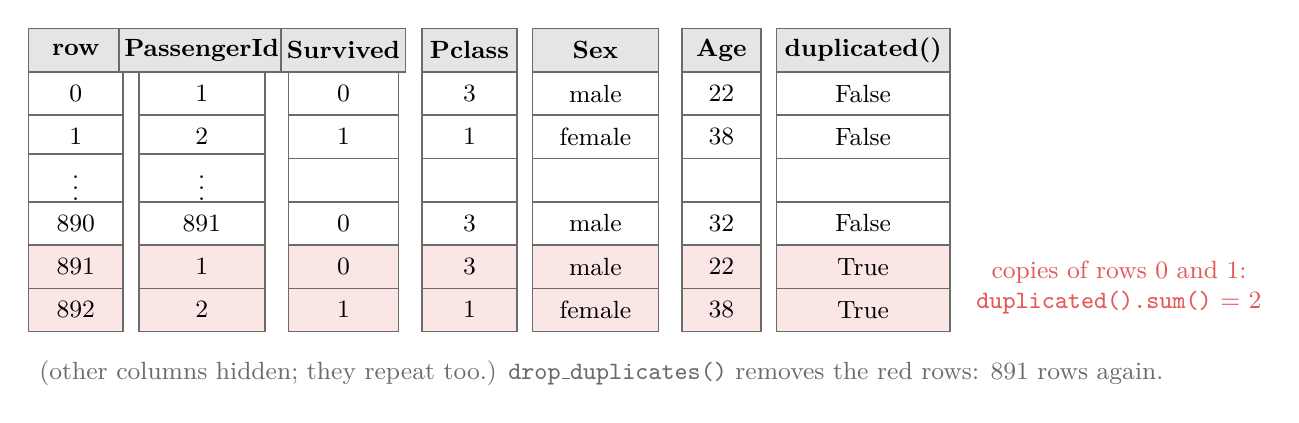
\begin{tikzpicture}[c/.style={draw=cgrey, minimum height=0.55cm, font=\sffamily\small, line width=0.6pt, inner sep=2pt},
  hd/.style={c, fill=black!10, font=\sffamily\small\bfseries}]
  \foreach \x/\w/\h in {0/1.2/row, 1.6/1.6/PassengerId, 3.4/1.4/Survived, 5.0/1.2/Pclass, 6.6/1.6/Sex, 8.2/1.0/Age, 10.0/2.2/duplicated()} \node[hd, minimum width=\w cm] at (\x, 0) {\h};
  \foreach \r/\rid/\pid/\s/\p/\sx/\a/\d/\f in {1/0/1/0/3/male/22/False/white, 2/1/2/1/1/female/38/False/white, 3/{\vdots}/{\vdots}/{}/{}/{}/{}/{}/white,
                                              4/890/891/0/3/male/32/False/white, 5/891/1/0/3/male/22/True/cred!15, 6/892/2/1/1/female/38/True/cred!15} {
    \node[c, minimum width=1.2cm, fill=\f] at (0, -0.55*\r) {\rid};
    \node[c, minimum width=1.6cm, fill=\f] at (1.6, -0.55*\r) {\pid};
    \node[c, minimum width=1.4cm, fill=\f] at (3.4, -0.55*\r) {\s};
    \node[c, minimum width=1.2cm, fill=\f] at (5.0, -0.55*\r) {\p};
    \node[c, minimum width=1.6cm, fill=\f] at (6.6, -0.55*\r) {\sx};
    \node[c, minimum width=1.0cm, fill=\f] at (8.2, -0.55*\r) {\a};
    \node[c, minimum width=2.2cm, fill=\f] at (10.0, -0.55*\r) {\d};
  }
  \node[note, anchor=west, text=cred] at (11.3, -3.02) {copies of rows 0 and 1:\\\texttt{duplicated().sum()} = 2};
  \node[note, anchor=west] at (-0.6, -4.1) {(other columns hidden; they repeat too.) \texttt{drop\_duplicates()} removes the red rows: 891 rows again.};
\end{tikzpicture}
\end{document}
